% =====================================================================
%  Presentación de sustentación — SmartDental
%  Beamer 16:9 · Asignatura: Gestión de Proyectos · Semana 8
%  Compilación: pdflatex presentacion && pdflatex presentacion
% =====================================================================
\documentclass[aspectratio=169,11pt]{beamer}
\usepackage[T1]{fontenc}
\usepackage[utf8]{inputenc}
\usepackage[spanish,es-noshorthands]{babel}
\usepackage[default,semibold]{sourcesanspro}
\usepackage[scale=0.86]{sourcecodepro}
\usepackage{fontawesome5}
\usepackage{ragged2e,etoolbox}
% Texto alineado a la izquierda en todo el documento, también dentro de columnas y cajas.
\AtBeginEnvironment{column}{\RaggedRight}
\AtBeginEnvironment{minipage}{\RaggedRight}
\setbeamertemplate{frame begin}{\RaggedRight}
\usepackage{booktabs,tabularx,array}
\usepackage{tikz}
\usetikzlibrary{positioning,arrows.meta,calc,fit,backgrounds,shadows.blur}

% ---------- Colores ----------
\definecolor{sdink}{HTML}{0D1B2A}
\definecolor{sdmuted}{HTML}{5B6676}
\definecolor{sdline}{HTML}{DDE3EA}
\definecolor{sdsoft}{HTML}{F3F6F9}
\definecolor{sdteal}{HTML}{0E9384}
\definecolor{sdmint}{HTML}{2FE0C8}
\definecolor{sdblue}{HTML}{1F5FBF}
\definecolor{sdsky}{HTML}{1E7BFF}
\definecolor{sdred}{HTML}{D64545}
\definecolor{sdamber}{HTML}{D08A1B}

% ---------- Tema ----------
\setbeamercolor{normal text}{fg=sdink,bg=white}
\setbeamercolor{structure}{fg=sdteal}
\setbeamertemplate{navigation symbols}{}
\setbeamertemplate{itemize items}{\color{sdteal}\small$\blacktriangleright$}
\setlength{\leftmargini}{1.1em}
\setbeamersize{text margin left=1cm,text margin right=1cm}
\hyphenpenalty=10000 \exhyphenpenalty=10000 \tolerance=2000 \emergencystretch=1em
\AtBeginDocument{\raggedright}

% Barra de progreso por bloques: 1 problema · 2 solución · 3 gestión · 4 diseño · 5 producto · 6 demo · 7 resultados
\newcommand{\bloque}{0}
\newcommand{\progreso}{%
  \begin{tikzpicture}[x=1cm,y=1cm]
    \foreach \i in {1,...,7} {
      \pgfmathsetmacro{\on}{\i<=\bloque ? 1 : 0}
      \ifdim\on pt>0pt \fill[sdteal,rounded corners=1pt] ({(\i-1)*0.62},0) rectangle ++(0.52,0.07);
      \else \fill[sdline,rounded corners=1pt] ({(\i-1)*0.62},0) rectangle ++(0.52,0.07); \fi
    }
  \end{tikzpicture}}
\setbeamertemplate{frametitle}{%
  \vspace*{0.55cm}%
  \begin{minipage}{\textwidth}
    \progreso\par\vspace{5pt}
    {\scriptsize\bfseries\color{sdteal}\MakeUppercase{\insertsectionhead}\par}\vspace{1pt}
    {\fontsize{22}{25}\selectfont\bfseries\color{sdink}\insertframetitle\par}
  \end{minipage}\vspace{0.1cm}}
\setbeamertemplate{footline}{\hbox to \paperwidth{\hfill{\color{sdmuted}\tiny\insertframenumber}\hspace{0.6cm}}\vspace{0.35cm}}

\tikzset{
  caja/.style={draw=sdline,line width=0.7pt,rounded corners=6pt,fill=white,align=center,font=\footnotesize,inner sep=7pt},
  cajaf/.style={rounded corners=8pt,fill=sdsoft,align=flush left,inner sep=10pt},
  flecha/.style={-{Latex[length=2.2mm]},draw=sdmuted!80,line width=0.8pt},
  sombra/.style={blur shadow={shadow blur steps=10,shadow xshift=0pt,shadow yshift=-2pt,shadow opacity=22}}}

% Icono en círculo de color
\newcommand{\icono}[3][sdteal]{\tikz[baseline=-0.6ex]\node[circle,fill=#1!14,text=#1,minimum size=#3,inner sep=0pt,font=\normalsize]{#2};}
% Cifra grande con icono
\newcommand{\cifra}[4][sdteal]{\begin{tikzpicture}\node[cajaf]{\begin{minipage}[t][2.35cm][t]{2.55cm}{\color{#1}\large #2}\par\vspace{2pt}{\fontsize{30}{32}\selectfont\bfseries\color{#1}#3\par}\vspace{3pt}{\scriptsize\color{sdmuted}#4\par}\end{minipage}};\end{tikzpicture}}
% Fila con icono, título y texto
\newcommand{\fila}[4][sdteal]{\begin{tikzpicture}[baseline=(t.north)]\node[circle,fill=#1!14,text=#1,minimum size=0.95cm,inner sep=0pt,font=\large](i){#2};\node[anchor=north west,text width=5.3cm,align=flush left,inner sep=0pt](t) at ([xshift=0.3cm,yshift=0.45cm]i.east){{\small\bfseries #3}\\[1pt]{\footnotesize\color{sdmuted}#4}};\end{tikzpicture}}
% Captura con sombra
\newcommand{\maqueta}[2][\linewidth]{\begin{tikzpicture}\node[inner sep=0pt,sombra,rounded corners=6pt,fill=white](m){\includegraphics[width=#1]{mockups/#2}};\end{tikzpicture}}

\begin{document}

% =====================================================================
%  PORTADA
% =====================================================================
{\setbeamertemplate{footline}{}
\begin{frame}[plain]
\begin{tikzpicture}[remember picture,overlay]
  \node[anchor=center,inner sep=0pt] at (current page.center) {
\includegraphics[width=\paperwidth,height=\paperheight]{mockups/cover_bg.jpg}};
  \foreach \i in {0,...,15}{
    \pgfmathsetmacro{\op}{(\i==7||\i==8)?0.95:0.15+0.03*abs(7.5-\i)}
    \draw[sdmint,line width=0.6pt,opacity=\op,rounded corners=1.2pt]
      ([xshift=1cm+\i*0.34cm,yshift=0.8cm]current page.south west) rectangle ++(0.22,0.22);}
\end{tikzpicture}
\vspace*{-0.2cm}
\begin{minipage}{0.44\textwidth}
{\scriptsize\color{white!55}\MakeUppercase{Universidad Nacional de Juliaca}\par}
\vspace{1.25cm}
{\scriptsize\bfseries\color{sdmint}\MakeUppercase{Sustentación · Gestión de Proyectos}\par}
\vspace{0.2cm}
{\fontsize{38}{40}\selectfont\bfseries\color{white}SmartDental\par}
\vspace{0.25cm}
{\normalsize\color{white!82}El consultorio dental, en orden:\\agenda, pacientes, odontograma, cotizaciones y caja en un solo sistema web.\par}
\vspace{0.6cm}
{\scriptsize\color{white!55}Ronal Abelin Larico Ccaso\quad·\quad 2026\par}
\end{minipage}
\end{frame}}

% =====================================================================
\section{El problema}\renewcommand{\bloque}{1}
\begin{frame}{El consultorio sigue en papel}
\begin{columns}[c]
\column{0.44\textwidth}
{\fontsize{19}{23}\selectfont\bfseries Fichas en papel, citas en un cuaderno y un WhatsApp personal.\par}
\vspace{0.35cm}
{\small\color{sdmuted}Funciona con pocos pacientes. Cuando el consultorio crece, la información se pierde y el tiempo también.\par}
\column{0.52\textwidth}
\fila[sdred]{\faCalendarTimes}{Citas olvidadas}{Sin confirmación ni seguimiento, el paciente no asiste y el horario se pierde.}\par\vspace{0.3cm}
\fila[sdred]{\faFolderOpen}{Historia clínica dispersa}{El odontograma en una hoja suelta no conserva la evolución de cada pieza.}\par\vspace{0.3cm}
\fila[sdred]{\faCalculator}{Presupuestos a mano}{Cada tratamiento se cotiza de memoria; el paciente no recibe un documento claro.}
\end{columns}
\end{frame}

% =====================================================================
\section{La solución}\renewcommand{\bloque}{2}
\begin{frame}{Todo el consultorio en un solo panel}
\begin{columns}[c]
\column{0.34\textwidth}
{\small\color{sdmuted}Objetivo general}\par
{\normalsize\bfseries Un sistema web multiclínica que centraliza la gestión clínica, administrativa y de comunicación.\par}
\vspace{0.35cm}
\begin{tikzpicture}[every node/.style={font=\footnotesize,anchor=west}]
  \foreach \ic/\t [count=\i] in {\faCalendarCheck/Agenda por profesional,\faTooth/Odontograma 2D y 3D,\faFileInvoiceDollar/Cotización automática,\faRobot/Asistente Denti con IA,\faIcon{shield-alt}/Datos aislados por clínica}{
    \node at (0,-\i*0.55) {\color{sdteal}\ic};
    \node at (0.45,-\i*0.55) {\t};}
\end{tikzpicture}
\column{0.64\textwidth}
\maqueta{resumen.jpg}
\end{columns}
\end{frame}

\begin{frame}{Objetivos del proyecto}
\begin{columns}[T]
\column{0.5\textwidth}
\fila{\faUserShield}{Acceso por roles}{Administrador, odontólogo y recepción, cada clínica con sus datos aislados.}\par\vspace{0.28cm}
\fila{\faTooth}{Módulos clínicos}{Agenda, ficha del paciente y odontograma con historial.}\par\vspace{0.28cm}
\fila{\faBoxes}{Organización}{Inventario con alertas, caja y atención por WhatsApp.}
\column{0.46\textwidth}
\fila{\faColumns}{Consola de plataforma}{Clínicas, planes, cobros y auditoría para el administrador general.}\par\vspace{0.28cm}
\fila{\faVial}{Verificación}{Pruebas automatizadas y validación con una clínica real.}
\end{columns}
\end{frame}

% =====================================================================
\section{Gestión del proyecto}\renewcommand{\bloque}{3}
\begin{frame}{Alcance y enfoque de trabajo}
\begin{columns}[c]
\column{0.3\textwidth}
{\small\bfseries\color{sdteal}\faCheckCircle\ Incluido}\par\vspace{3pt}
{\footnotesize Sitio público y acceso por roles\\Panel de clínica (11 secciones)\\Consola de plataforma\\Cotización y tarifario\\Asistente con IA\par}
\vspace{0.3cm}
{\small\bfseries\color{sdmuted}\faTimesCircle\ Fuera de esta versión}\par\vspace{3pt}
{\footnotesize\color{sdmuted}Facturación electrónica\\Pagos en línea\\App móvil nativa\par}
\column{0.66\textwidth}
\centering
\begin{tikzpicture}[font=\footnotesize,scale=0.78,every node/.append style={transform shape}]
  \node[circle,fill=sdteal,text=white,minimum size=1.7cm,font=\small\bfseries,align=center] (c) at (0,0) {Incremento\\funcional};
  \foreach \ang/\ic/\t in {90/\faClipboardList/Backlog priorizado,0/\faCode/Desarrollo,-90/\faVial/Pruebas,180/\faEye/Revisión en el navegador}{
    \node[circle,fill=sdsoft,text=sdteal,minimum size=1.05cm,font=\large] (n\ang) at (\ang:2.25) {\ic};
    \node[font=\scriptsize\bfseries,text=sdink] at ($(n\ang)+(\ang:0.95)$) {\t};}
  \draw[flecha,sdteal] (n90) to[bend left=30] (n0);
  \draw[flecha,sdteal] (n0) to[bend left=30] (n-90);
  \draw[flecha,sdteal] (n-90) to[bend left=30] (n180);
  \draw[flecha,sdteal] (n180) to[bend left=30] (n90);
\end{tikzpicture}

{\scriptsize\color{sdmuted}Enfoque ágil e incremental (Scrum adaptado a un desarrollador): cada vuelta deja una versión que compila y se prueba.}
\end{columns}
\end{frame}

\begin{frame}{Cronograma: junio a noviembre de 2026}
\centering
\begin{tikzpicture}[x=0.058cm,y=0.5cm,font=\scriptsize]
  \foreach \m/\x in {Junio/0,Julio/30,Agosto/61,Septiembre/92,Octubre/122,Noviembre/153}{
    \fill[sdsoft] (\x,0.55) rectangle ++(29,0.55);
    \node[anchor=west,text=sdmuted,font=\scriptsize\bfseries] at (\x+1,0.83) {\m};
    \draw[sdline] (\x,0.55) -- (\x,-9.6);}
  \foreach \t/\a/\b/\y/\c in {
    Planificación y diseño/0/19/0/sdink,
    Plataforma multiclínica/13/27/-1/sdteal,
    Módulos clínicos/21/75/-2/sdteal,
    Consola de plataforma/20/91/-3/sdteal,
    Inventario{,} caja y WhatsApp/27/111/-4/sdteal,
    Odontograma 2D y 3D/92/131/-5/sdteal,
    Cotización y asistente con IA/150/158/-6/sdsky,
    Pruebas y seguridad/30/158/-7/sdblue,
    Documentación y sustentación/136/162/-8/sdblue}{
    \node[anchor=east,text=sdink] at (-2,\y) {\t};
    \fill[\c,rounded corners=2.5pt] (\a,\y-0.3) rectangle (\b,\y+0.3);}
  \foreach \x/\l/\an in {13/Esquema inicial/north east,27/Multiclínica/north west,143/Flujos aislados/north east,158/IA y tarifario/north west}{
    \fill[sdred] (\x,-9.15) +(0,0.22) -- +(0.22*5,0) -- +(0,-0.22) -- +(-0.22*5,0) -- cycle;
    \node[anchor=\an,text=sdmuted,font=\tiny] at (\x,-9.45) {\l};}
\end{tikzpicture}
\end{frame}

\begin{frame}{Recursos y riesgos}
\begin{columns}[c]
\column{0.42\textwidth}
\centering
\begin{tikzpicture}[x=1.35cm,y=1.35cm]
  \foreach \i in {0,1,2} \foreach \j in {0,1,2} {
    \pgfmathtruncatemacro{\lvl}{(\i+1)*(\j+1)}
    \ifnum\lvl>5 \fill[sdred!30,rounded corners=4pt] (\i,\j) rectangle ++(1.25,1.25);
    \else\ifnum\lvl>2 \fill[sdamber!24,rounded corners=4pt] (\i,\j) rectangle ++(1.25,1.25);
    \else \fill[sdteal!16,rounded corners=4pt] (\i,\j) rectangle ++(1.25,1.25); \fi\fi}
  \tikzset{r/.style={circle,fill=sdink,text=white,font=\scriptsize\bfseries,inner sep=0pt,minimum size=0.52cm}}
  % (impacto, probabilidad): R1 (3,2) R5 (3,2) R2 (2,2) R6 (2,2) R3 (2,3) R7 (1,2)
  \node[r] at (2.35,1.62) {R1}; \node[r] at (2.85,1.62) {R5};
  \node[r] at (1.35,1.62) {R2}; \node[r] at (1.85,1.62) {R6};
  \node[r] at (1.6,2.62) {R3};
  \node[r] at (0.62,1.62) {R7};
  \node[rotate=90,font=\scriptsize,text=sdmuted] at (-0.3,1.95) {Probabilidad $\rightarrow$};
  \node[font=\scriptsize,text=sdmuted] at (1.95,-0.3) {Impacto $\rightarrow$};
\end{tikzpicture}
\column{0.54\textwidth}
\footnotesize
\begin{tabularx}{\linewidth}{@{}p{0.55cm}Xr@{}}
\textbf{R1} & Fuga de datos entre clínicas & \textcolor{sdteal}{\textbf{Corregido}}\\
\textbf{R2} & Cambios en servicios de terceros & \textcolor{sdteal}{\textbf{Corregido}}\\
\textbf{R3} & Crecimiento del alcance & \textcolor{sdteal}{\textbf{Controlado}}\\
\textbf{R5} & Datos clínicos sensibles & \textcolor{sdteal}{\textbf{Controlado}}\\
\textbf{R6} & WhatsApp depende de Meta & \textcolor{sdamber}{\textbf{Abierto}}\\
\textbf{R7} & Rendimiento visual y 3D & \textcolor{sdteal}{\textbf{Corregido}}\\
\end{tabularx}
\vspace{0.3cm}
{\scriptsize\color{sdmuted}\faUser\ 1 desarrollador para todos los roles\\ \faHospital\ 1 clínica usuaria para validar\\ \faCloud\ Supabase y servicios en la nube\par}
\end{columns}
\end{frame}

% =====================================================================
\section{Análisis y diseño}\renewcommand{\bloque}{4}
\begin{frame}{Arquitectura del sistema}
\centering
\begin{tikzpicture}[node distance=0.4cm and 1.2cm,
  capa/.style={rounded corners=8pt,minimum height=3.3cm,text width=3.1cm,align=center,inner sep=8pt},
  pieza/.style={rounded corners=5pt,fill=white,draw=sdline,text width=2.6cm,align=left,font=\scriptsize,inner sep=5pt}]
  \node[capa,fill=sdink,text=white] (nav) {{\Huge\faDesktop}\\[6pt]{\small\bfseries Navegador}\\[2pt]{\scriptsize\color{white!75}React 18 + Vite\\Panel de clínica\\Consola de plataforma}};
  \node[capa,fill=sdteal!10,right=1.3cm of nav,text width=3.4cm,minimum height=3.6cm] (sb) {};
  \node[font=\scriptsize\bfseries,text=sdteal] at ([yshift=-0.32cm]sb.north) {SUPABASE};
  \node[pieza] (a) at ([yshift=0.6cm]sb.center) {\color{sdteal}\faKey\ \color{sdink}\textbf{Auth} · sesiones};
  \node[pieza,below=0.12cm of a] (b) {\color{sdteal}\faDatabase\ \color{sdink}\textbf{PostgreSQL} · RLS};
  \node[pieza,below=0.12cm of b] (c) {\color{sdteal}\faServer\ \color{sdink}\textbf{Edge Functions}};
  \node[capa,fill=sdsoft,right=1.3cm of sb] (ext) {{\Huge\color{sdsky}\faRobot}\\[6pt]{\small\bfseries Servicios}\\[2pt]{\scriptsize\color{sdmuted}Modelo de lenguaje\\WhatsApp Cloud API}};
  \draw[flecha,line width=1.2pt] (nav) -- (sb);
  \draw[flecha,line width=1.2pt,{Latex[length=2.2mm]}-{Latex[length=2.2mm]}] (sb) -- (ext);
\end{tikzpicture}

\vspace{0.3cm}
{\small Cada consulta solo ve las filas de \textbf{su clínica} y de \textbf{su rol}: la regla vive en PostgreSQL, no en la pantalla.}
\end{frame}

% =====================================================================
\section{El producto}\renewcommand{\bloque}{5}
\begin{frame}{Módulos para el día a día}
\centering
\begin{tikzpicture}
  \node[inner sep=0pt,sombra,rounded corners=6pt,fill=white] (a) at (0,0) {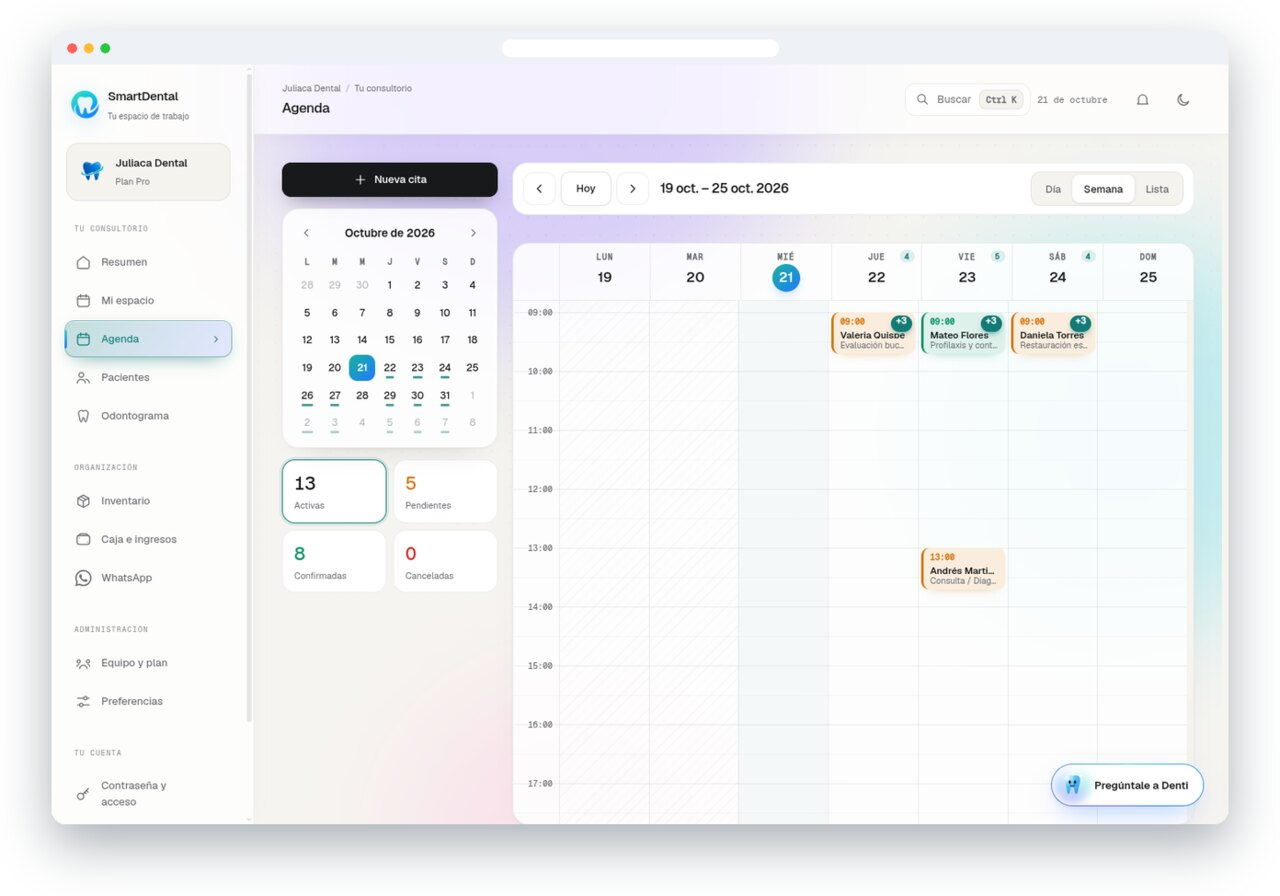
\includegraphics[width=6.8cm]{mockups/agenda.jpg}};
  \node[inner sep=0pt,sombra,rounded corners=6pt,fill=white,anchor=north west] (b) at ([xshift=0.35cm,yshift=-0.15cm]a.north east) {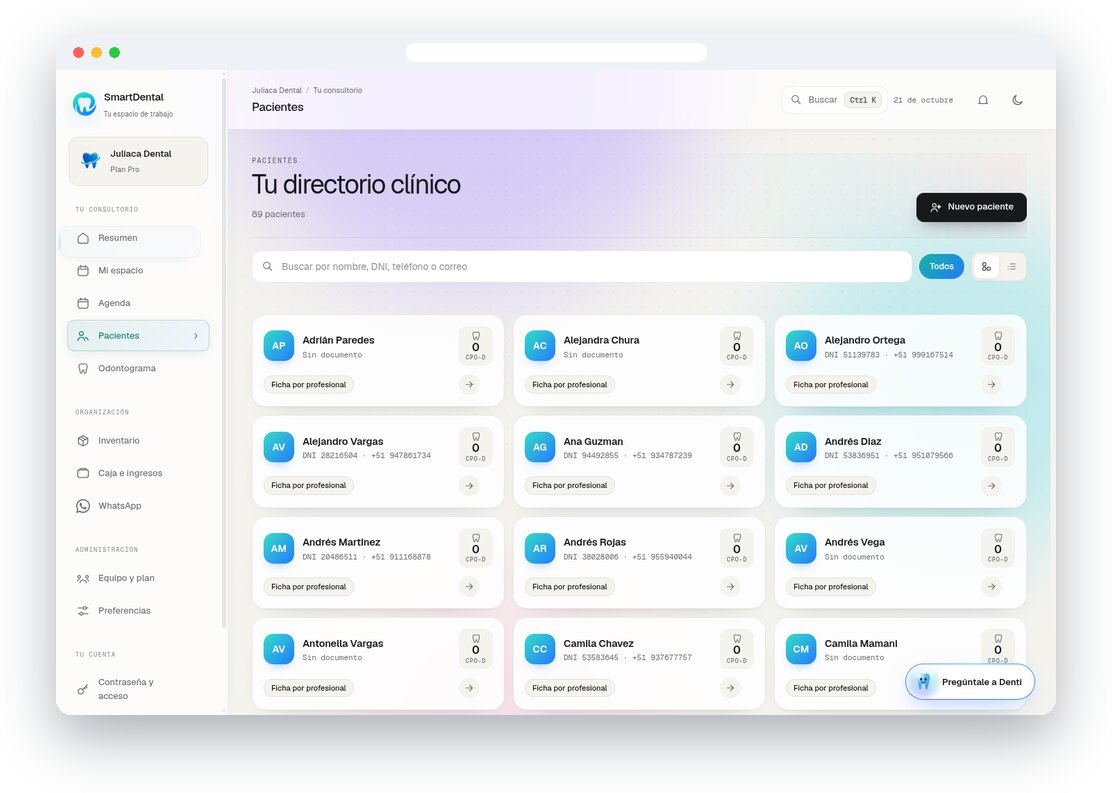
\includegraphics[width=3.6cm]{mockups/pacientes.jpg}};
  \node[inner sep=0pt,sombra,rounded corners=6pt,fill=white,anchor=north west] (c) at ([yshift=-0.55cm]b.south west) {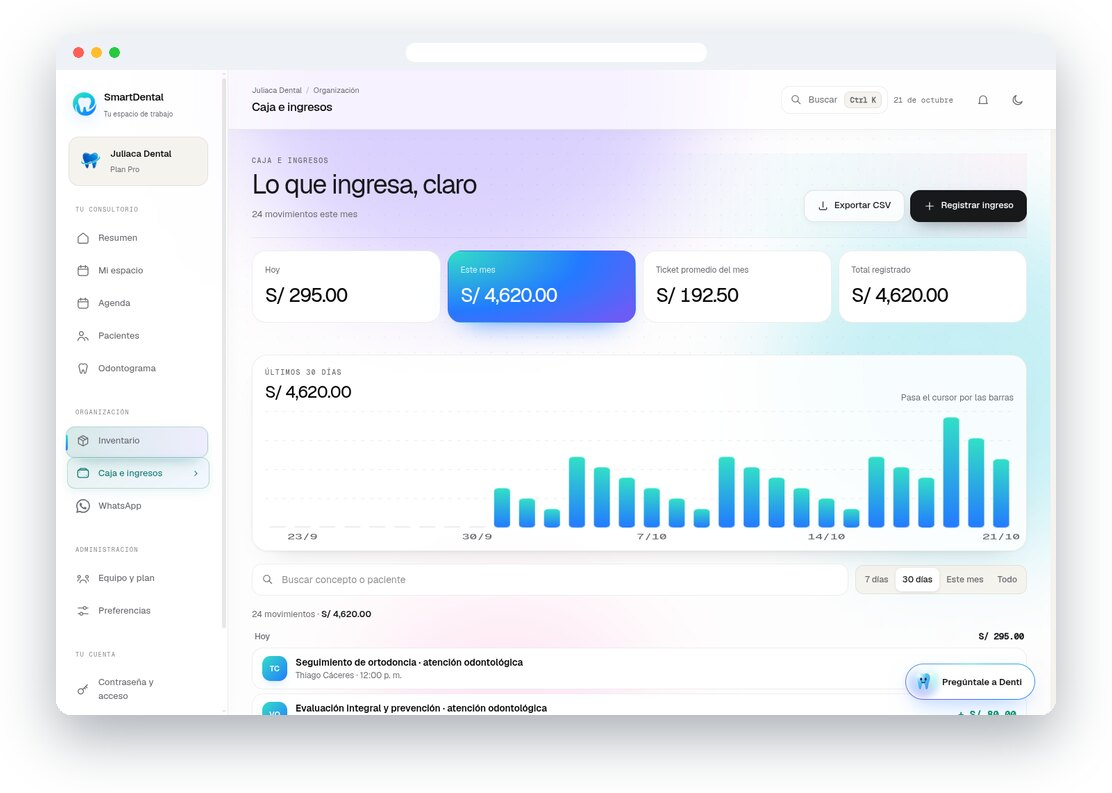
\includegraphics[width=3.6cm]{mockups/caja.jpg}};
  \node[font=\scriptsize\bfseries,anchor=north west,text=sdink] at ([yshift=-0.08cm]a.south west) {\color{sdteal}\faIcon{calendar-alt}\ Agenda semanal con citas superpuestas agrupadas};
  \node[font=\scriptsize\bfseries,anchor=south west,text=sdink] at ([yshift=0.06cm]b.north west) {\color{sdteal}\faUsers\ Pacientes};
  \node[font=\scriptsize\bfseries,anchor=south west,text=sdink] at ([yshift=0.06cm]c.north west) {\color{sdteal}\faCashRegister\ Caja e ingresos};
\end{tikzpicture}
\end{frame}

\begin{frame}{Odontograma profesional, en 2D y en 3D}
\begin{columns}[c]
\column{0.3\textwidth}
\begin{itemize}\small\setlength{\itemsep}{5pt}
  \item Notación \textbf{FDI}: permanente, temporal o mixta.
  \item Marcas por pieza y por cara.
  \item \textcolor{sdred}{\textbf{Rojo}} hallazgo · \textcolor{sdblue}{\textbf{azul}} tratamiento.
  \item Índices \textbf{CPO-D} y \textbf{ceo-d}.
  \item Arcada 3D coloreada por estado.
\end{itemize}
\column{0.68\textwidth}
\begin{tikzpicture}
  \node[inner sep=0pt,sombra,rounded corners=6pt,fill=white] (a) at (0,0) {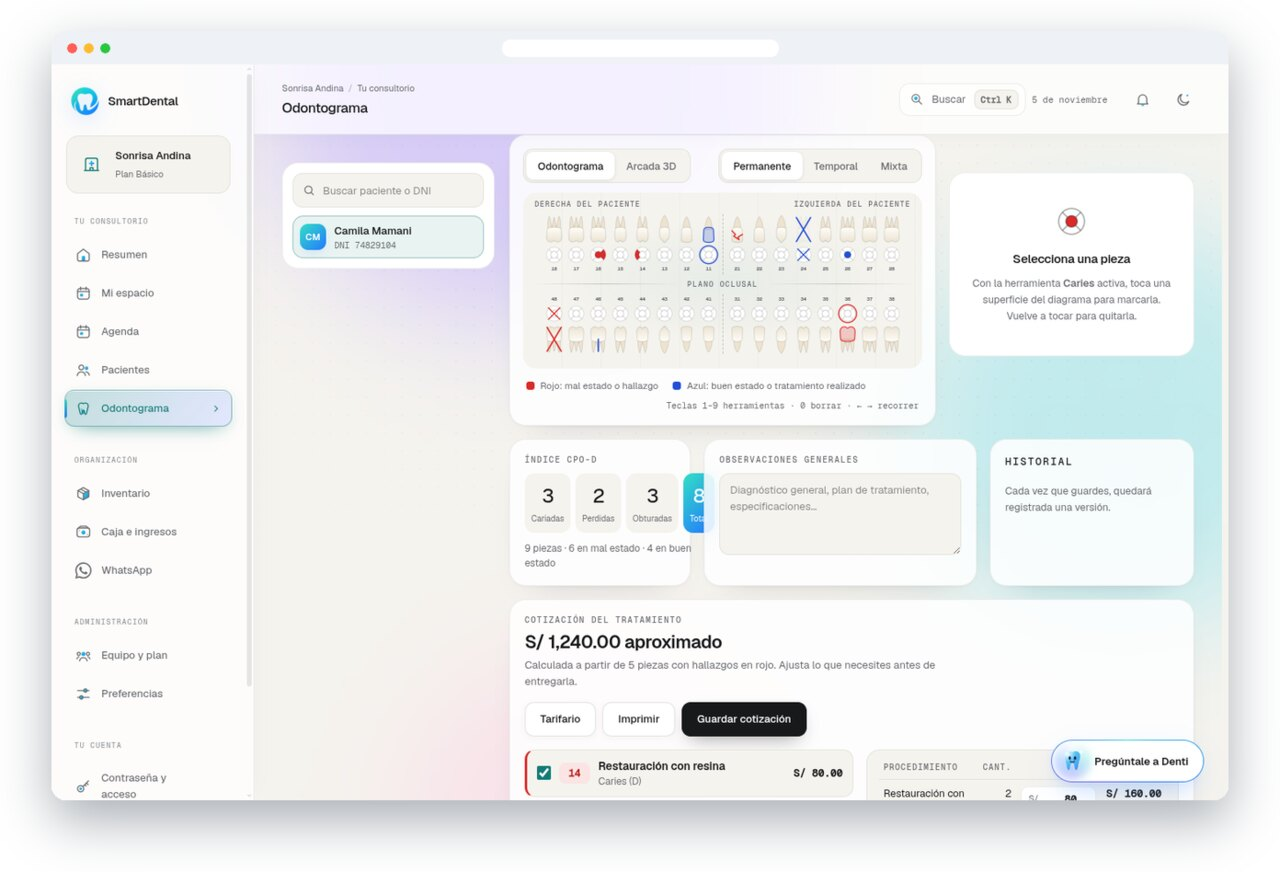
\includegraphics[width=6.1cm]{mockups/odo2d.jpg}};
  \node[inner sep=0pt,sombra,rounded corners=6pt,fill=white] at ($(a.south east)+(-1.2,0.55)$) {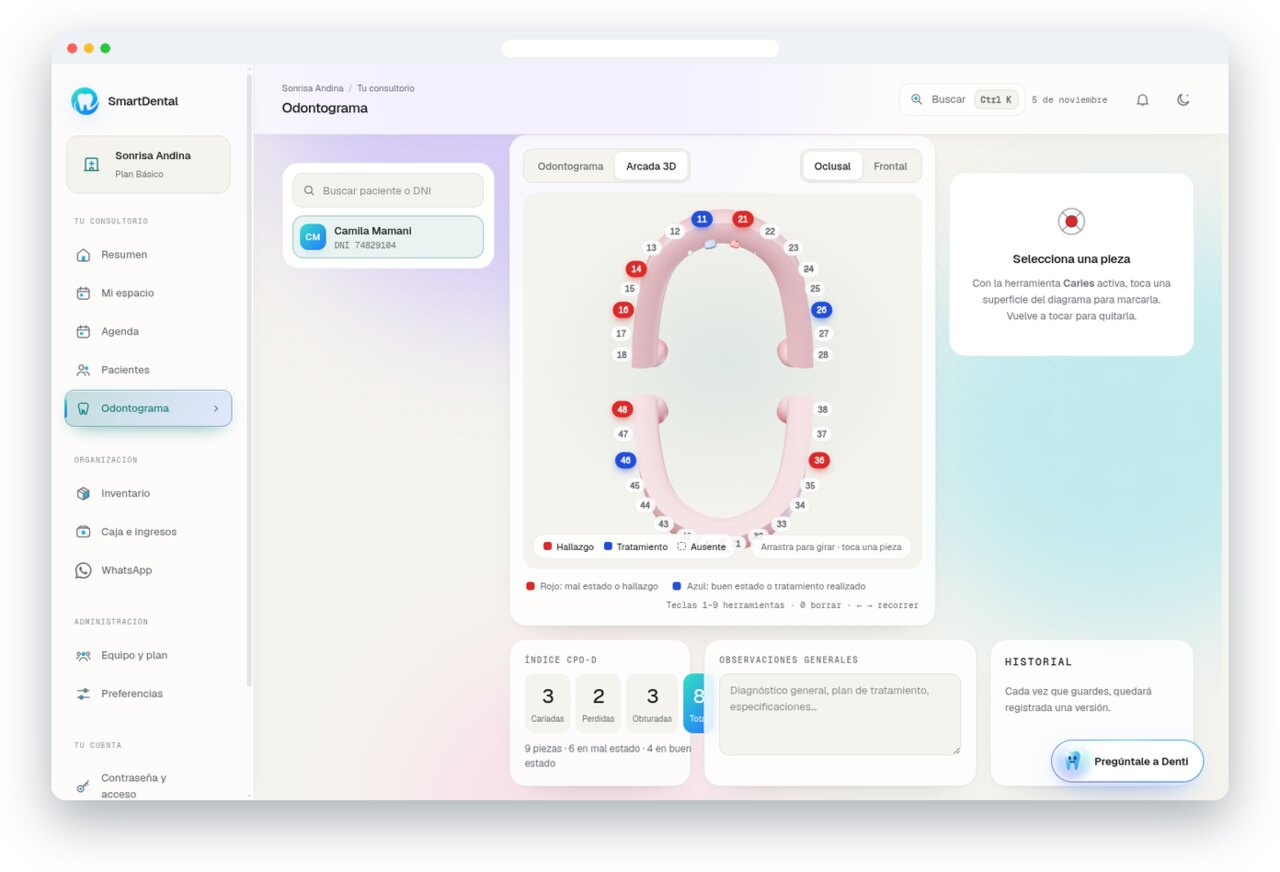
\includegraphics[width=4.2cm]{mockups/odo3d.jpg}};
\end{tikzpicture}
\end{columns}
\end{frame}

\begin{frame}{Cotización desde el odontograma}
\begin{columns}[c]
\column{0.42\textwidth}
\begin{tikzpicture}[paso/.style={rounded corners=7pt,fill=sdsoft,text width=4.4cm,align=flush left,inner sep=6pt,font=\scriptsize}]
  \node[paso] (p1) {{\color{sdred}\bfseries\faTooth\ Hallazgo en rojo}\\Caries en las caras O y M de la pieza 16};
  \node[paso,below=0.22cm of p1] (p2) {{\color{sdteal}\bfseries\faClipboardCheck\ Procedimiento}\\Resina + 1 cara adicional};
  \node[paso,below=0.22cm of p2] (p3) {{\color{sdteal}\bfseries\faTags\ Tarifario de la clínica}\\S/~80 + S/~30};
  \node[paso,below=0.22cm of p3,fill=sdink,text=white] (p4) {{\bfseries\faFileInvoiceDollar\ Total aproximado}\\{\large\bfseries S/~110} · imprimible en PDF};
  \foreach \a/\b in {p1/p2,p2/p3,p3/p4} \draw[flecha,sdteal,line width=1pt] (\a) -- (\b);
\end{tikzpicture}
\column{0.56\textwidth}
\maqueta[0.95\linewidth]{quote.jpg}

\vspace{0.12cm}
{\scriptsize\color{sdmuted}Solo se cobra lo pendiente (rojo), con el tarifario de cada clínica.}
\end{columns}
\end{frame}

\begin{frame}{Denti: asistente con IA}
\begin{columns}[c]
\column{0.36\textwidth}
\centering
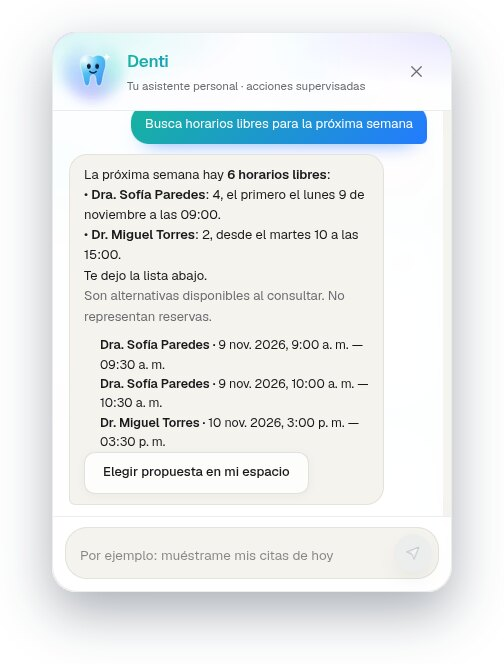
\includegraphics[height=4.9cm]{mockups/denti.jpg}
\column{0.6\textwidth}
{\footnotesize Pregúntale como a un colega: \textit{«busca horarios libres la próxima semana»}.\par}
\vspace{0.2cm}
\fila{\faLock}{Usa tus permisos}{Lee la agenda con tu sesión: un odontólogo solo ve su propia agenda.}\par\vspace{0.12cm}
\fila{\faUserSecret}{Datos mínimos}{Al modelo nunca llegan DNI, teléfono ni identificadores internos.}\par\vspace{0.12cm}
\fila{\faHandPaper}{Tú confirmas}{No cambia citas por su cuenta: una cancelación es solo una propuesta.}
\end{columns}
\end{frame}

% =====================================================================
\section{Demostración}\renewcommand{\bloque}{6}
\begin{frame}{Demostración en vivo}
\vspace{0.4cm}
\centering
\begin{tikzpicture}[x=2.25cm,
  num/.style={circle,fill=sdteal,text=white,font=\large,minimum size=1.15cm,inner sep=0pt},
  txt/.style={text width=1.9cm,align=center,font=\footnotesize}]
  \draw[sdline,line width=2pt] (0,0) -- (5,0);
  \foreach \i/\ic/\t in {0/\faIcon{sign-in-alt}/Inicio de sesión,1/\faUserPlus/Registrar un paciente,2/\faCalendarPlus/Reservar y confirmar la cita,3/\faTooth/Marcar el odontograma,4/\faFileInvoiceDollar/Cotizar el tratamiento,5/\faRobot/Preguntar a Denti}{
    \node[num] at (\i,0) {\ic};
    \node[txt,anchor=north] at (\i,-0.75) {\t};
    \node[font=\scriptsize\bfseries,text=sdteal] at (\i,0.85) {\pgfmathparse{int(\i+1)}0\pgfmathresult};}
\end{tikzpicture}

\vspace{0.9cm}
{\footnotesize\color{sdmuted}\faInfoCircle\ Clínica con datos de demostración: no se muestran pacientes reales.}
\end{frame}

% =====================================================================
\section{Resultados}\renewcommand{\bloque}{7}
\begin{frame}{Resultados}
\centering
\cifra{\faVial}{114}{pruebas automatizadas correctas}\hfill
\cifra{\faCheckDouble}{7}{flujos validados con una clínica real}\hfill
\cifra{\faUsersCog}{4}{roles con datos aislados}\hfill
\cifra[sdsky]{\faFlagCheckered}{4/5}{objetivos cumplidos; WhatsApp depende de Meta}
\vspace{0.5cm}

\begin{columns}[T]
\column{0.32\textwidth}
{\small\bfseries\color{sdteal}\faLightbulb\ Aprendizaje}\par
{\footnotesize La seguridad multiclínica se diseña en la base de datos, no en la interfaz.}
\column{0.32\textwidth}
{\small\bfseries\color{sdteal}\faExclamationTriangle\ Dificultad}\par
{\footnotesize Revisar el propio trabajo sin equipo: lo compensaron las pruebas automatizadas.}
\column{0.32\textwidth}
{\small\bfseries\color{sdteal}\faRoute\ Próximos pasos}\par
{\footnotesize Recordatorios por WhatsApp, kárdex y comprobantes en PDF.}
\end{columns}
\end{frame}

% =====================================================================
{\setbeamertemplate{footline}{}
\setbeamercolor{background canvas}{bg=sdink}
\begin{frame}[plain]
\begin{tikzpicture}[remember picture,overlay]
  \shade[left color=sdink,right color=sdink!75!sdteal] (current page.north west) rectangle (current page.south east);
\end{tikzpicture}
\vspace*{0.4cm}
\hspace*{0.2cm}\begin{minipage}{0.86\textwidth}
{\scriptsize\bfseries\color{sdmint}CONCLUSIÓN\par}
\vspace{0.3cm}
{\fontsize{26}{31}\selectfont\bfseries\color{white}SmartDental reemplaza el papel y el Excel por un sistema que todo el equipo comparte.\par}
\vspace{0.5cm}
{\normalsize\color{white!78}La gestión por incrementos, con una definición de terminado y pruebas automatizadas, permitió entregar un sistema funcional y verificable aun concentrando todos los roles en una sola persona.\par}
\vspace{1.1cm}
{\fontsize{30}{32}\selectfont\bfseries\color{white}Gracias.\ }{\large\color{sdmint}¿Preguntas?\par}
\vspace{0.25cm}
{\footnotesize\color{white!55}\faLink\ github.com/garou7ro/SmartDental\par}
\end{minipage}
\end{frame}}

\end{document}
